% Perry Mills, Luke Snyder
% Database Management Systems project

\documentclass{article}      % Specifies the document class

                             % The preamble begins here.
\title{CSCE 4523 DBMS \\
\large Project}  % Declares the document's title.
\author{Perry Mills, Luke Snyder}      % Declares the author's name.
\date{April 23, 2017}      % Deleting this command produces today's date.

\usepackage{enumitem}
\usepackage{amsmath}
\usepackage{amssymb}
\usepackage{needspace}
\usepackage{hyperref}

\usepackage{graphicx}
\graphicspath{ {screenshots/} }

\begin{document}             % End of preamble and beginning of text.

\maketitle                   % Produces the title.

\section*{Included Files}
The following files are included in the submission:
\begin{description}
\item [CreateTables.sh] MySQL table definitions.
\item [build\_odbc.bash] Compile backend .cpp files.
\item [config.php] Path definition.
\item [index.php] Landing page.
\item [odbc\_db.cpp, .h] Interface to MySQL database.
\item [odbc\_insert\_course.cpp, .php] Handle function 2.
\item [odbc\_insert\_enrollment.cpp, .php] Handle function 3.
\item [odbc\_insert\_student.cpp, .php] Handle function 1.
\item [odbc\_reinitialize.cpp] Reset tables.
\item [odbc\_select\_deptCourses.cpp, .php] Handle function 5.
\item [odbc\_select\_studentCourses.cpp, .php] Handle function 6.
\item [odbc\_select\_students.cpp, .php] Handle function 4.
\end{description}

\section*{Compilation}
The assignment can be unpacked then built with GCC by executing \textbf{build\_odbc.bash}.
The landing page can be accessed at:
\begin{itemize}
\item \url{http://csce.uark.edu/~ls008/StudentRegistration/}
\item \url{http://csce.uark.edu/~pwm001/DBProject/StudentRegistration/}
\end{itemize}
The program has been compiled and tested in the Turing environment with connections from
Firefox and Google Chrome.

\section*{Design}
The web front is written in PHP, hosted via Turing's Apache server.
HTML forms are used to gather input from the user and make calls to the back end,
which is written in C++.
The back end uses the provided ODBC interface (which was used in the previous assignment)
to interact with a MySQL database, also hosted on Turing.

For portability, the path to which PHP calls are made to the backend is read from a single
\textbf{config.php} file (one line).
The database login information is read in the \textbf{odbc\_db.cpp} constructor (three lines).
With changes on just these four lines, the project can be ported to another location/user.

One bug-fix was made to the C++ version of the provided ODBC.
Within \textbf{odbc\_db::disConnect()}, a check is now made to ensure the resultSet
is not null before attempting to delete it.
Without this check, segmentation faults could and would occur regularly when making a 
connection without a valid query.

Additionally, a function was added to reinitialize the tables from the web front.
This returns the database to fresh tables with several sample tuples in each.

\section*{Database tables}
The database is designed with a generic university in mind.
In many cases where characters are used, it is to accomodate schools which
include letters in their naming system.
Following the sample design, the database includes three tables:
\subsection*{Student}
The Student table includes a unique identifier StudentId,
the student's name and the student's major.
The StudentId field supports up to 9 characters, which supports UA's 9-digit standard
as well as other alpha-numeric systems.
Because it is a unique identifier, it is the primary key.
The StudentName field allows 50 characters, enough for most cases.
Similarly, the Major field allows room for long degree names.
None of the attributes may be null, and "Undeclared" can be used in place of NULL for Major.
\subsection*{Course}
The Course table identifies courses by the combination of Department code and course number.
For example, ECON 3404 is distinct from ECON 2004 and HUMN 3404,
which are a different course within the same department and a different course outside the
department which coincidentally uses the same course number, respectively.
Course number allows up to 5 characters, supporting courses such as 3404L or other conventions.
Title and Credit Hour fields can be null, for flexibility in adding courses for which
not all details are finalized.
\subsection*{Enrollment}
An enrollment consists of pairing a student with a distinct course.
Students are identified by StudentId, while courses have a composite key.
As a result, all included attributes compose the primary key, and all attributes are foreign
keys to the other tables (accordingly, no attributes may be null).
Each foreign key constraint cascades deletion, so that if a course is
removed all the associated students are unenrolled, and so that if a student is removed,
that student is no longer enrolled in any courses.

\section*{Error checking}
The error testing for this project was extensive and consists of the following:
\begin{enumerate}
\item Adding a student page
	\begin{itemize}
	\item The StudentId, Name, or Major cannot be empty (validated through HTML form).
	\item The StudentId must consist of only numeric digits
		(validated through PHP isValidId() function).
	\end{itemize}
\item Adding a course page
	\begin{itemize}
	\item The DeptCode, CourseNum, Title, or CreditHours cannot be empty
		(validated through HTML form).
	\item The CreditHours must be a positive integer (validated through HTML form).
	\end{itemize}
\item Adding an enrollment application page
	\begin{itemize}
	\item The StudentId, DeptCode, and CourseNum cannot be empty
		(validated through HTML form).
	\item Since each of the fields references a student and course in the respective
		tables, if any of the fields references non-existing data, an exception is
		thrown on the server side, generating a user-friendly error.  
	\end{itemize}
\item Viewing courses for a given department page
	\begin{itemize}
	\item The DeptCode cannot be empty (validated through HTML form).
	\item If a non-existing DeptCode is entered, an exception is thrown on the
		server side, generating a user-friendly error.
	\end{itemize}
\item Viewing courses for a given StudentId page
	\begin{itemize}
	\item The StudentId cannot be empty (validated through HTML form).
	\item If a non-existing StudentId is entered, or one which is not enrolled in any
		classes, an exception is thrown on the server side, generating a
		user-friendly error.
	\end{itemize}
\end{enumerate}


\section*{Screenshots}
\begin{enumerate}
\item Landing page

	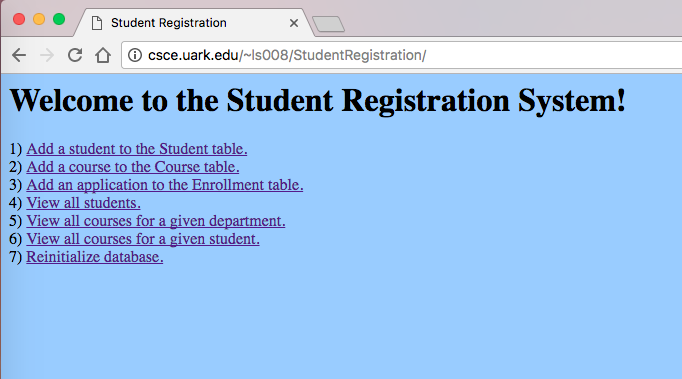
\includegraphics[width=\textwidth]{HomeScreen}


\item Inserting a student

	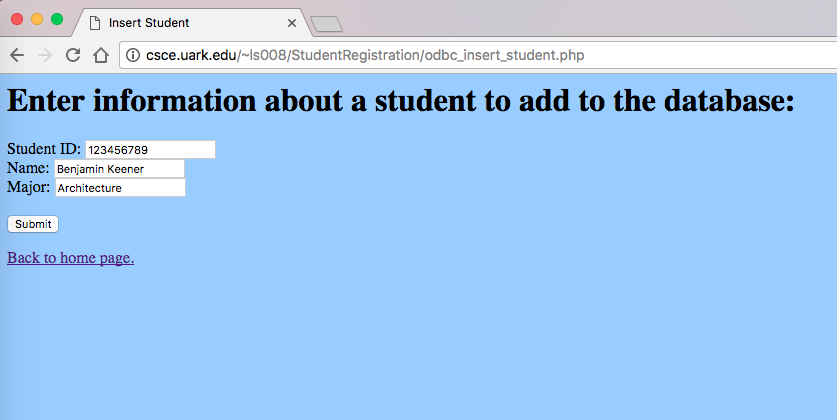
\includegraphics[width=\textwidth]{InsertStudentBefore}
	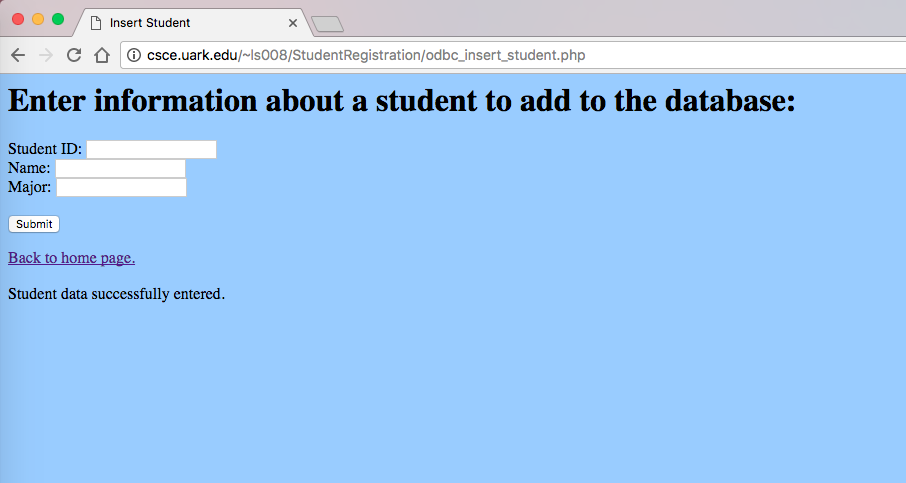
\includegraphics[width=\textwidth]{InsertStudentAfter}


\item Inserting a course

	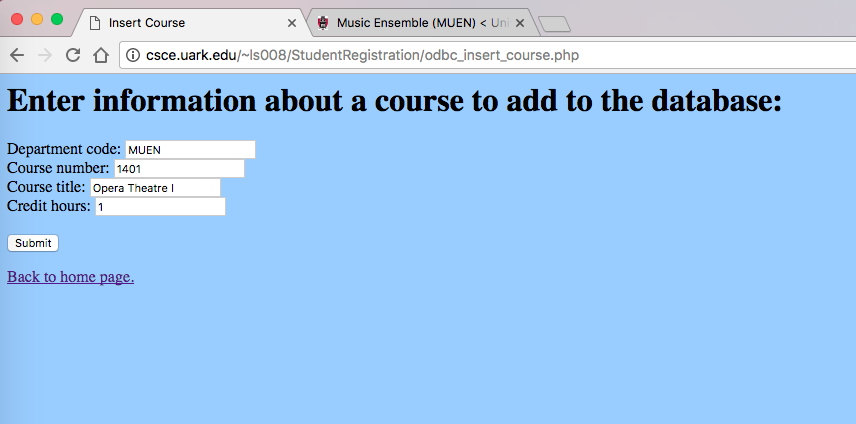
\includegraphics[width=\textwidth]{InsertCourseBefore}
	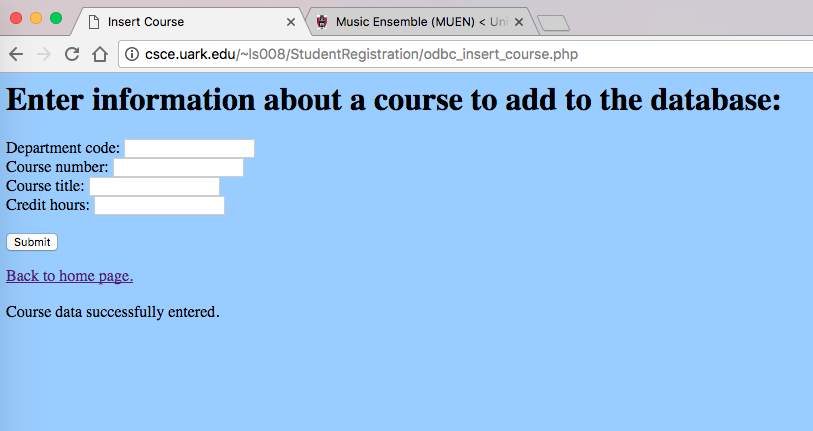
\includegraphics[width=\textwidth]{InsertCourseAfter}


\item Enrolling a student

	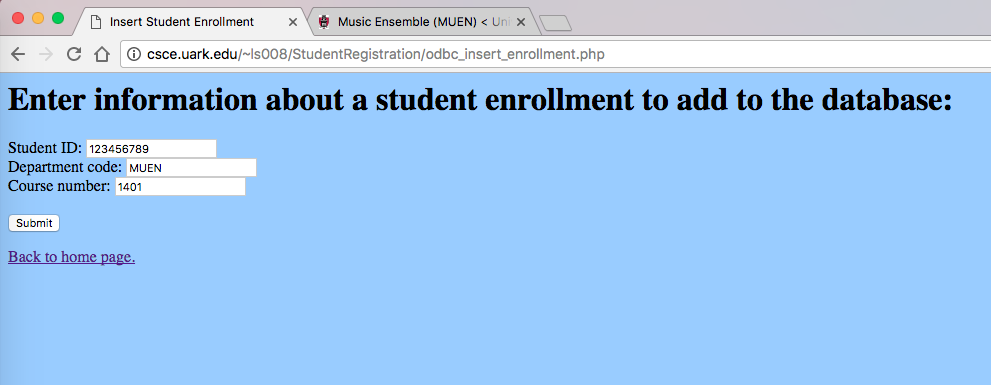
\includegraphics[width=\textwidth]{InsertEnrollmentBefore}
	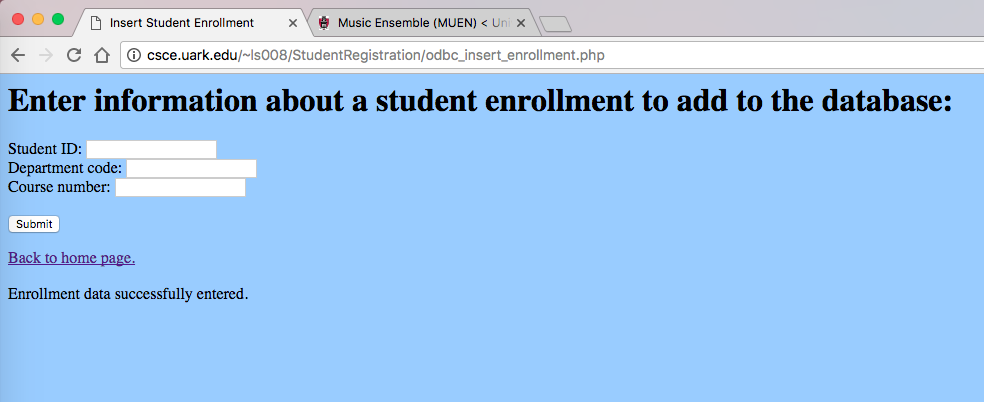
\includegraphics[width=\textwidth]{InsertEnrollmentAfter}


\item View all students

	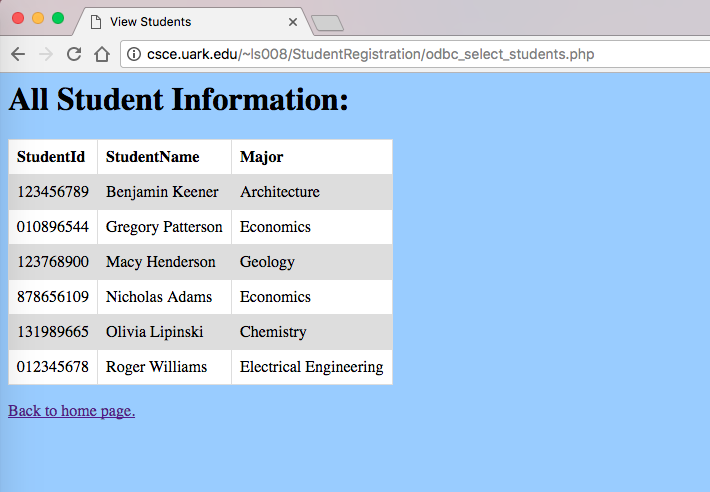
\includegraphics[width=\textwidth]{ViewStudents}


\item View all courses offered by a department

	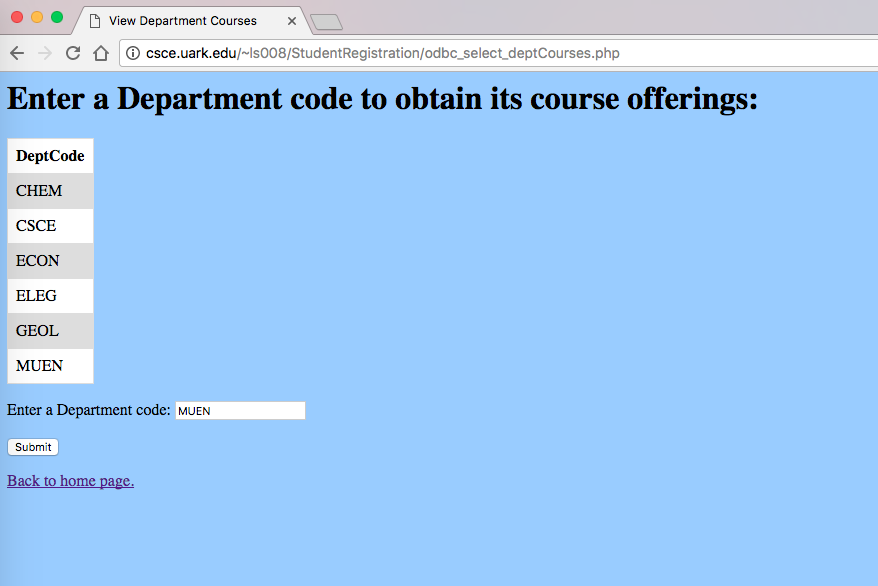
\includegraphics[width=\textwidth]{ViewDepartmentCoursesBefore}
	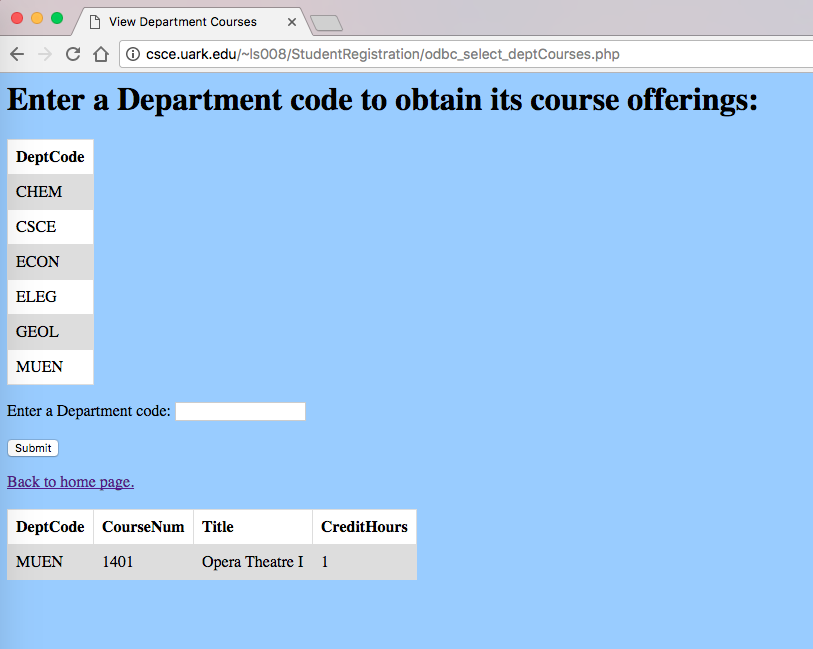
\includegraphics[width=\textwidth]{ViewDepartmentCoursesAfter}


\item View all enrollments for a student

	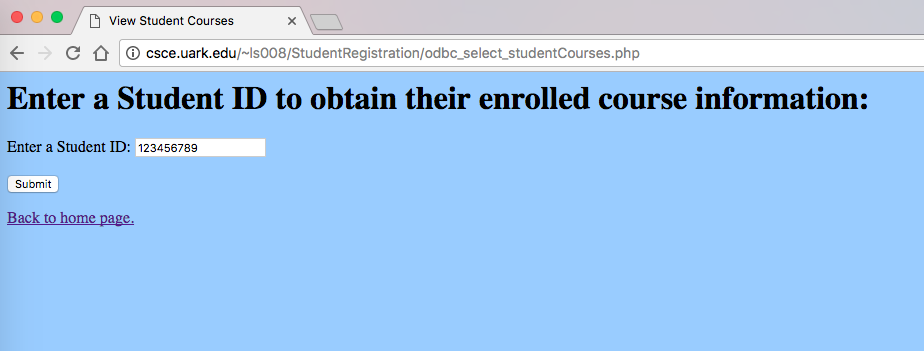
\includegraphics[width=\textwidth]{ViewStudentCoursesBefore}
	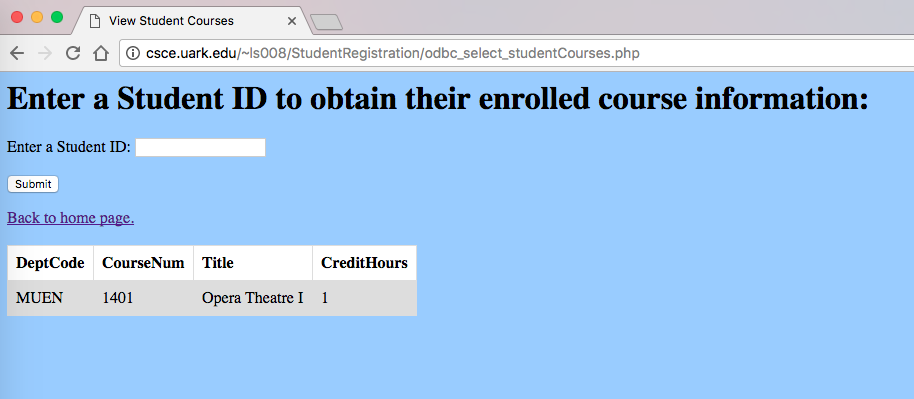
\includegraphics[width=\textwidth]{ViewStudentCoursesAfter}
\end{enumerate}



\end{document}               % End of document.
